\documentclass[aspectratio=169]{beamer}
\usepackage{etex} % fixes new-dimension error
\usepackage{lmodern}
\usepackage[T1]{fontenc}

\usepackage{graphicx,amsmath}
\usepackage{stmaryrd} % cf. interleave
\usepackage{booktabs}
\usepackage{amscd}
\usepackage{multicol}
\usepackage[absolute,overlay]{textpos}
\usepackage{alltt}
\usepackage{proof}
\usepackage{subcaption}
\usepackage{tikz}
\usepackage{tikz-cd}
\usepackage[new]{old-arrows}
\usepackage[all]{xy}
\usepackage{pgfplots}
\usepackage{textcomp}

%------ using color ---------------------------------------------------------
%\newrgbcolor{goldenrod}{.80392 .60784 .11373}
%\newrgbcolor{darkgoldenrod}{.5451 .39608 .03137}
%\newrgbcolor{brown}{.15 .15 .15}
%\newrgbcolor{darkolivegreen}{.33333 .41961 .18431}
\definecolor{goldenrod}{rgb}{.80392,.60784,.11373}
\definecolor{darkgoldenrod}{rgb}{.5451,.39608,.03137}
\definecolor{brown}{rgb}{.15,.15,.15}
\definecolor{darkolivegreen}{rgb}{.33333,.41961,.18431}
\definecolor{darkgreen}{rgb}{0,0.6,0}
\definecolor{myGray}{gray}{0.85}
%


% \newcommand{\red}[1]{\textcolor{red!80!black}{#1}\xspace}
% \newcommand{\blue}[1]{\textcolor{blue}{#1}\xspace}
% \newcommand{\gold}[1]{\textcolor{darkgoldenrod}{#1}\xspace}
\newcommand{\grey}[1]{\textcolor{myGray}{#1}\xspace}
\def\laplace#1#2{*\txt{\mbox{ \fcolorbox{black}{myGray}{$\begin{array}{c}\mbox{#1}\\\\#2\\\\\end{array}$} }}}
\newenvironment{bluein}{\blue}{\black\hskip -2.5pt}

%------ contexts  ---------------------------------------------------------

\newtheorem{defi}{Defini\cao}[section]
\newtheorem{defi*}{Defini\cao}
\newtheorem{lema*}{Lema}
\newenvironment{lsbcom}
      {\footnotesize  \hrule ~\\ ~\\ {\bf \sc Nota:} }
      {\hrule  ~\\ ~\\  \normalsize}
      
\newenvironment{lsbcomi}
      {\footnotesize  \hrule ~\\ ~\\ {\bf \sc Note:} }
      {\hrule  ~\\ ~\\  \normalsize}
      
\newenvironment{demo}%
     {\vspace{-5mm}\noindent {\bf Prova:}}%
    {\par \nopagebreak  \noindent \fimdemo \vspace{3mm} }
\newenvironment{demoi}%
     {\vspace{-5mm}\noindent {\bf Proof:}}%
    {\par \nopagebreak  \noindent \fimdemo \vspace{3mm} }


% \newcommand{\N}{\ensuremath{\mathbb{N}}\xspace}
% \newcommand{\Z}{\ensuremath{\mathbb{Z}}\xspace}
% \newcommand{\R}{\ensuremath{\mathbb{R}}\xspace}

\newcommand{\cR}{\ensuremath{\mathcal{R}}\xspace}

% \newcommand{\set}[1]{\left\{ #1 \right\}} % {a,b,...z}
\def\bang{{!}}
\def\deff{\stackrel{\rm def}{=}}          % Function definition symbol
%\def\deff{\, :=\, }          % Function definition symbol


\def\always{\boxempty}
\def\eventual{\Diamond}
\def\nexts{\bigcirc}
\def\until{\mathbin{\mathcal U}}




%------ CCS          -----------------------------------------%
\def\ppe{\mathbin{\vartriangleright}}
\def\kcomp{\mathbin{\boldsymbol{\bullet}}}
%\def\qcomp{\mathbin{\boldsymbol{;}}}
\def\ssp{\textsc{skip}}
\def\fim{\dagger}
%\def\ppe{\gg}
\def\ff{\ensuremath{\mi{f\!f}}\xspace}
\def\tt{\ensuremath{\mi{t\!t}}\xspace}
\def\cnil{\mathbf{0}}
\def\cpf#1#2{#1 . #2}                           % a.P
\def\cou#1#2{#1 \mathbin{+} #2}                 % P + Q
%\def\crt#1#2{\mathbin{#1 \setminus_{#2}}}       % P \ A
%\def\crtt#1#2{\mathbin{#1 \setminus\!\setminus_{#2}}}       % P \ A
%\def\crt#1#2{\mathsf{new}\, #2\;  #1}       % P \ A
\def\crt#1#2{#1 \backslash #2}       % P \ A
%\def\crn#1#2{\{#2\}\, #1}                  % P[f]

\def\crn#1#2{\mathbin{#1[#2]}}                  % P[f]
\def\couit#1#2{\Sigma_{#1}#2}                  %  + i=1,n
\def\cpar#1#2{#1 \mid #2}                       %  |
\def\ctpar#1#2{#1 \parallel #2}                       %  |
\def\cpars#1#2#3{#1 \mid_{#3} #2}               %  |S
\def\ffix#1#2{\underline{fix}~(#1\, =\, #2)}  % fix X
\def\fffix#1#2#3{\underline{fix}_{#1}~(#2\, =\, #3)}  % fix X
\def\tfix#1#2{\underline{\Tilde{fix}}~(\Tilde{#1}\, =\, \Tilde{#2})}  % fix X
%\def\ainv#1{\Bar{#1}}                   % ~ a
\def\ainv#1{\overline{#1}}                   % ~ a
\def\cif#1#2{\fuc{if}\, #1\, \fuc{then}\, #2}
\def\ccif#1#2#3{\fuc{if}\, #1\, \fuc{then}\, #2\, \fuc{else}\, #3}

\def\fres#1#2{#1 \restriction #2}                

\def\mean#1{\mathopen{[\![}#1\mathclose{]\!]}}
\def\llbracket{\mathopen{[\![}}
\def\rrbracket{\mathopen{]\!]}}

\def\cfree#1{\fuc{fn} (#1)}
\def\cbound#1{\fuc{bn} (#1)}
\def\anew#1{\overline{#1}\mathsf{new}\, } 
\def\transitatau{\rtran{\tau}}
\def\transitaa{\rtran{a}}


% 2015




%%%%%%%%%%%%%%%% NUNO reconf


\def\trans#1{\stackrel{#1}{\longrightarrow}}
\def\TS#1{\mathcal{G}(#1)}
\def\TSn#1{\mathcal{G}_{nodes}(#1)}




%--------------------
%--- by jose 2016 ---
%--------------------

\newcommand{\myblock}[1]{\begin{beamercolorbox}[dp=1ex,center,rounded=true]%
  {postit} {\large \textbf{#1}} \end{beamercolorbox}}%
\def\trans#1{\xrightarrow{#1}}  % - a - > 
\def\Trans#1{\stackrel{#1}{\Longrightarrow}} % =a=> 
\def\transtau{\xrightarrow{\tau}}  % - a - > 


%\newcommand{\evm}[1]{\langle #1 \rangle\,\fi}
%\newcommand{\alm}[1]{[#1]\,}
\newcommand{\evm}[1]{\if\relax\detokenize{#1}\relax 
  \Diamond \else\langle #1 \rangle\fi}
\newcommand{\alm}[1]{\if\relax\detokenize{#1}\relax 
  \boxempty \else[#1]\fi}

\newcommand{\myparagraph}[1]{\medskip\noindent\textbf{#1}~~}



% Listing
\lstset{
  language=Scala,
  basicstyle=\ttfamily\footnotesize, % overriding size
  commentstyle=\sffamily\color{green!60!black},
}
% \lstset{%language=Java
% %  ,basicstyle=\footnotesize
%   ,columns=fullflexible %space-fexible
%   ,keepspaces
% %  ,numberstyle=\tiny
%   ,mathescape=true
%   ,showstringspaces=false
% %  ,morekeywords={refract,global,local,on-change}
%   ,morecomment=[l]{\%}
%   ,commentstyle=\sl\sffamily\color{gray}\scriptsize
%   ,basicstyle=\ttfamily\relsize{-0.5}
%   ,keywordstyle=\bf\sffamily\color{purple}
% %  ,emphstyle=\it\sffamily\color{blue!80!black}
%   ,emphstyle=\bfseries\itshape\color{blue!80!black}
%   ,emphstyle={[2]\itshape\color{red!70!black}}%\underbar}
%   ,stringstyle=\color{darkgreen}
%   ,alsoletter={-,||,+,<>,&&,=>}
%   ,literate=*{->}{{{\color{red!70!black}$\to$}}}{1}
%              {.}{{{\color{red!70!black}.}}}{1}
%              {+}{{{\color{red!70!black}+}}}{1}
%              {*}{{{\color{red!70!black}*}}}{1}
%              {\#}{{{\color{red!70!black}\#}}}{1}
%   ,emph={act,proc,init,sort}
%   ,emph={[2]block,hide,comm,rename,allow,||,<>,sum,&&,=>}
% %  ,emphstyle={[2]\color{blue}}2
%   ,framerule=1pt
%   ,backgroundcolor=\color{black!2}
%   ,rulecolor=\color{black!30}
%   ,frame=tblr
%   ,xleftmargin=4pt
%   ,xrightmargin=4pt
%   ,captionpos=b
% %  ,belowcaptionskip=\medskipamount
%   ,aboveskip=\baselineskip
%   ,floatplacement=htb
% }
\lstdefinestyle{bash}{literate=*}
% \newcommand{\code}[1]{\lstinline[basicstyle=\ttfamily\relsize{-0.5},keywordstyle=\bf\sffamily\color{purple},columns=fullflexible,keepspaces]�#1�}
\newcommand{\code}[1]{\lstinline[columns=fullflexible,basicstyle=\ttfamily\small\color{blue},keepspaces]�#1�}
\newcommand{\mcode}[1]{\text{\code{#1}}}
\newcommand{\bash}[1]{\lstinline[basicstyle=\ttfamily\relsize{-0.5}\color{darkgreen},keywordstyle=\bf\sffamily\color{purple},columns=fullflexible,keepspaces,literate=*]�#1�}


%%%%%
% Named environments (no counters) 
\newenvironment{theorem}[2][Theorem]{\begin{trivlist}
\item[\hskip \labelsep {\bfseries #1}\hskip \labelsep {\bfseries #2.}]}{\end{trivlist}}
\newenvironment{lemma}[2][Lemma]{\begin{trivlist}
\item[\hskip \labelsep {\bfseries #1}\hskip \labelsep {\bfseries #2.}]}{\end{trivlist}}
%\newenvironment{exercise}[2][Exercise]{\begin{trivlist}
%\item[\hskip \labelsep {\bfseries #1}\hskip \labelsep {\bfseries #2.}]}{\end{trivlist}}
\newenvironment{problem}[2][Problem]{\begin{trivlist}
\item[\hskip \labelsep {\bfseries #1}\hskip \labelsep {\bfseries #2.}]}{\end{trivlist}}
\newenvironment{question}[2][Question]{\begin{trivlist}
\item[\hskip \labelsep {\bfseries #1}\hskip \labelsep {\bfseries #2.}]}{\end{trivlist}}
\newenvironment{corollary}[2][Corollary]{\begin{trivlist}
\item[\hskip \labelsep {\bfseries #1}\hskip \labelsep {\bfseries #2.}]}{\end{trivlist}}
 
% Environments with counters
\newtheoremstyle{myplain} {8mm}% (Space above)
{3mm}% (Space below)
{}% (Body font)
{}% (Indent amount)
{\bfseries\large}% (Theorem head font)
{.}% (Punctuation after theorem head)
{.5em}% (Space after theorem head)2
{}% (Theorem head spec (can be left empty, meaning �normal�))

\theoremstyle{myplain}
\newtheorem{myExercise}{Exercise}

\theoremstyle{definition} % no italics
\newtheorem{subexercise}{}[myExercise]

\newcommand{\ex}[1]{\begin{myExercise}#1\end{myExercise}}
\newcommand{\subex}[1]{\begin{subexercise}#1\end{subexercise}}

\newcommand{\mytikz}[2][]{\medskip\centerline{\begin{tikzpicture}[#1]#2\end{tikzpicture}}\medskip}



%%%%% REO %%%%
\pgfdeclarelayer{background}
\pgfdeclarelayer{threadground}
\pgfsetlayers{background,threadground,main}

\usepackage{pgfplots}

% thickness of the lines
\tikzstyle{border}   = [thick]
\tikzstyle{reodist}    = [node distance=15mm]

% nodes and I/O
\tikzstyle{reonode}  = [border,circle,inner sep=1.5pt,reodist]
\tikzstyle{mixed}    = [reonode, line width=0, %draw=black,
%                        outer color=black,inner color=black!20
                        shading=ball,ball color=black]
\tikzstyle{boundary} = [reonode,draw=black,fill=white]
\tikzstyle{point}    = [reonode,draw=black,fill=black,inner sep=0.5pt]
\tikzstyle{io}       = [border,rectangle,draw=black,fill=white,inner sep=3.25pt,node distance=0.75cm]
\tikzstyle{ioblack}  = [border,rounded corners=0,rectangle,draw=black,
    fill=black,inner sep=3.25pt,node distance=0.75cm]
\tikzstyle{comp}     = [border,rectangle,draw=black,fill=white,inner sep=3.25pt,reodist]
\tikzstyle{token} = [inner sep=0.8mm,regular polygon,regular polygon sides=5,draw=black, fill=#1]
\newcommand{\token}{\tikz \node[token=green!70!black] {};\xspace}


%% animations
\tikzstyle{animflow}=[blue,draw opacity=0.2,line width=2.7mm,line cap=round,line join=round]                   
\tikzstyle{animnf}=[postaction=decorate,line width=0,draw opacity=0,
                  decoration={markings,mark=at position #1 with 
                  {\node[regular polygon,regular polygon sides=3,rotate=30,draw=red,draw opacity=0.5,line width=1.5pt,line cap=round,line join=round, rounded corners=0.5pt,
                  transform shape,inner sep=1.3pt]{};}}]
\tikzstyle{animfflow}=[blue!20,line width=2.7mm,line cap=round,line join=round]                   


% channels
\tikzstyle{channel}=[border,>=stealth]
\tikzstyle{sync}=[channel,->]
\tikzstyle{lossy}=[channel,->,dashed]
\tikzstyle{sdrain}=[channel,>-<]
\tikzstyle{sspout}=[channel,<->]
\tikzstyle{fifo}=[channel,->,
                  postaction=decorate,
                  decoration={markings,mark=at position 0.5 with 
                  {\node[rectangle,draw=black,fill=white,rounded corners=0,
                  transform shape,minimum width=6mm]{#1};}}]
\tikzstyle{fifos}=[channel,->,
                  postaction=decorate,
                  decoration={markings,mark=at position 0.5 with 
                  {\node[rectangle,draw=black,fill=white,rounded corners=0,
                  transform shape,minimum width=4mm]{#1};}}]
\tikzstyle{fifocol}=[channel,->,
                  postaction=decorate,
                  decoration={markings,mark=at position 0.5 with 
                  {\node[rectangle,draw=black,fill=#1,rounded corners=0,
                  transform shape,minimum width=6mm]{};}}]
\tikzstyle{vare}=[channel,->,
                  postaction=decorate,
                  decoration={markings,mark=at position 0.5 with 
                  {\node[rectangle,draw=black,fill=white,rounded corners=3,
                  transform shape,minimum width=6mm]{#1};}}]
\tikzstyle{varf}=[channel,->,
                  postaction=decorate,
                  decoration={markings,mark=at position 0.5 with 
                  {\node[rectangle,draw=black,fill=black,rounded corners=3,
                  transform shape,minimum width=6mm]{#1};}}]
\tikzstyle{filter}=[channel,->,
                  decorate,rounded corners=0,
                  decoration={zigzag,segment length=1.3mm, 
                  pre length=4mm,post length=4mm,#1}]
\tikzstyle{lfilter}=[channel,->,
                  decorate,rounded corners=0,
                  decoration={zigzag,segment length=1.3mm, 
                  pre length=#1,post length=#1}]
\tikzstyle{llfilter}=[channel,->,
                  decorate,rounded corners=0,
                  decoration={zigzag,segment length=1.3mm, 
                  pre length=#1,post length=#1}]
\tikzstyle{transf}=[channel,->,
                  postaction=decorate,
                  decoration={markings,mark=at position 0.45 with 
                  {\node[isosceles triangle,draw=black,fill=white,rounded corners=0,
                  transform shape,inner sep=2pt,#1]{};}}]
\tikzstyle{clossy}=[channel,->,dashed,
                  postaction=decorate,
                  decoration={markings,mark=at position 0.5 with 
                  {\node[sloped]{!};}}]
\tikzstyle{pdrain}=[channel,>-<,
                  postaction=decorate,
                  decoration={markings,
                    mark=at position 0.5 with
                      {\draw[channel,-]
                        (-2pt,-3pt) -- (-2pt,3pt) [transform shape]
                        (2pt,-3pt) -- (2pt,3pt) [transform shape];},
                    mark=at position 0.25 with {\node[sloped]{!};}}]

\tikzstyle{adrain}=[channel,>-<,
    postaction=decorate,
    decoration={markings,mark=at position 0.5 with
    {\draw[channel,-] (-2pt,-3pt) -- (-2pt,3pt) [transform shape]
                      (2pt,-3pt) -- (2pt,3pt) [transform shape];}}]
\tikzstyle{aspout}=[channel,<->,
    postaction=decorate,
    decoration={markings,mark=at position 0.5 with
    {\draw[channel,-] (-2pt,-3pt) -- (-2pt,3pt) [transform shape]
                      (2pt,-3pt) -- (2pt,3pt) [transform shape];}}]


% connector box
\tikzstyle{connector}=[fill=black!10,rounded corners]

\newcommand{\reoconnector}[2][]{
  \begin{tikzpicture}[line join=round,#1]
  #2
  \end{tikzpicture}
}

%%% LOTS OF WORK for an exclusive router.

% \pgfdeclareshape{circle cross}
% {
%   \inheritsavedanchors[from=circle] % this is nearly a circle
%   \inheritanchorborder[from=circle]
%   \inheritanchor[from=circle]{north}
%   \inheritanchor[from=circle]{north west}
%   \inheritanchor[from=circle]{north east}
%   \inheritanchor[from=circle]{center}
%   \inheritanchor[from=circle]{west}
%   \inheritanchor[from=circle]{east}
%   \inheritanchor[from=circle]{mid}
%   \inheritanchor[from=circle]{mid west}
%   \inheritanchor[from=circle]{mid east}
%   \inheritanchor[from=circle]{base}
%   \inheritanchor[from=circle]{base west}
%   \inheritanchor[from=circle]{base east}
%   \inheritanchor[from=circle]{south}
%   \inheritanchor[from=circle]{south west}
%   \inheritanchor[from=circle]{south east}
%   \inheritbackgroundpath[from=circle]
%   \foregroundpath{
%     \centerpoint%
%     \pgf@xc=\pgf@x%
%     \pgf@yc=\pgf@y%
%     \pgfutil@tempdima=\radius%
%     \pgfmathsetlength{\pgf@xb}{\pgfkeysvalueof{/pgf/outer xsep}}%  
%     \pgfmathsetlength{\pgf@yb}{\pgfkeysvalueof{/pgf/outer ysep}}%  
%     \ifdim\pgf@xb<\pgf@yb%
%       \advance\pgfutil@tempdima by-\pgf@yb%
%     \else%
%       \advance\pgfutil@tempdima by-\pgf@xb%
%     \fi%
%     \pgfpathmoveto{\pgfpointadd{\pgfqpoint{\pgf@xc}{\pgf@yc}}{\pgfqpoint{-0.707107\pgfutil@tempdima}{0.707107\pgfutil@tempdima}}}
%     \pgfpathlineto{\pgfpointadd{\pgfqpoint{\pgf@xc}{\pgf@yc}}{\pgfqpoint{0.707107\pgfutil@tempdima}{-0.707107\pgfutil@tempdima}}}
%     \pgfpathmoveto{\pgfpointadd{\pgfqpoint{\pgf@xc}{\pgf@yc}}{\pgfqpoint{-0.707107\pgfutil@tempdima}{-0.707107\pgfutil@tempdima}}}
%     \pgfpathlineto{\pgfpointadd{\pgfqpoint{\pgf@xc}{\pgf@yc}}{\pgfqpoint{0.707107\pgfutil@tempdima}{0.707107\pgfutil@tempdima}}}
%   }
% }

% \tikzstyle{exrouter} = [border,inner sep=1.5mm,
%      reodist,draw=black,fill=white,circle cross]
% \tikzstyle{smallexrouter} = [border,inner sep=1.0mm,
%      reodist,draw=black,fill=white,circle cross]

\tikzstyle{exrouter}=[border,draw=black,circle,path picture={
  \draw[black](path picture bounding box.south east) -- (path picture bounding box.north west) (path picture bounding box.south west) -- (path picture bounding box.north east);}]


%--------- Setting headers ---------------
\usepackage{fancyhdr}
\usepackage{lastpage}
% \pagestyle{plain}
\pagestyle{fancy}

\newcommand{\setHeader}[2]{
  \newcommand{\myHeader}{
    \thispagestyle{empty}
    \begin{center}
      \bfseries
      {\Large #1}\\[2mm]
      \LOGO DCC-FCUP, University of Porto\\
      Jos\'{e} Proen\c{c}a\\[2mm]
      #2
    \end{center}

    % \noindent
    % Number: \rule{20mm}{0.5pt}
    % Name: \rule{116.5mm}{0.5pt}

    % \noindent
    % \hrulefill\\[0mm]
    % {\footnotesize
    % \textbf{Recall:}\\
    % \begin{minipage}{0.67\textwidth}
    %   $f(n) = \mathcal{O}(g(n))$
    %     if there exist $n0,c>0$ such that $\forall n\geq n0: f(n) \leq c \times g(n)$
    %   \\[1mm]
    %   $f(n) = \Omega(g(n))$
    %     if there exist $n0,c>0$ such that $\forall n\geq n0: f(n) \geq c \times g(n)$
    %   \\[1mm]
    %   $f(n) = \Theta(g(n))$
    %     if $f(n) = \mathcal{O}(g(n))$ and $f(n) = \Omega(g(n))$
    %   \\[1mm]
    %   Master Theorem: if $T(n)=aT(n/b) + cn^k$ then $T(N)$ is:
    %   \\\hspace*{3mm}$[\Theta(n^k)$ if $a < b^k$]
    %   ~~~[$\Theta(n^k\log n)$ if $a=b^k$]
    %   ~~~[$\Theta(n^{\log_b a}$) if $a > b^k$]
    % \end{minipage}
    % \begin{minipage}{0.31\textwidth}
    % % \begin{align*}
    %     $\sum_{i=1}^n i ~=~ \frac{n(n+1)}{2}$
    %     \\[3mm]
    %     ${\sum_{i=0}^n x^i} ~=~
    %           {\frac{x^{n+1}-1}{x-1}}$
    %     \\[3mm]
    %     ${\sum_{i=1}^n i \times x^{i-1}} ~=~ 
    %           {\frac{n\times x^{n+1}-(n+1)\times x^n +1}{(x-1)^2}}$
    % % \end{align*}
    % \end{minipage}
    % \\[2mm]
    % Answer below each question. If you need more space, use the empty space at the end of the exam.
    % \\[-1mm]If needed ask for a new paper.
    % \\[-6mm]
    % }

    \noindent
    \hrulefill
  }

  \newcommand{\newExamPage}{
    \clearpage
    \thispagestyle{empty}
    % ~
    % \newpage
    \begin{center}
      \bfseries
      {\Large #1} (continuation -- \thepage/\pageref{LastPage})\\[2mm]
      DCC-FCUP, University of Porto,
      Jos\'{e} Proen\c{c}a,
      #2
    \end{center}

    % \noindent
    % % \hrulefill
    % % \\[2mm]
    % Number: \rule{20mm}{0.5pt}
    % Name: \rule{116.5mm}{0.5pt}
  }

  \renewcommand{\headrulewidth}{.4mm} % header line width
  \fancyhf{}
  % \fancyhfoffset[L]{1cm} % left extra length
  % \fancyhfoffset[R]{1cm} % right extra length
  \rhead{\thepage/\pageref{LastPage}}
  \lhead{\bfseries #1}
  \rfoot{}
}
%-----------------------------------------


%%% Misc

\def\pv#1#2{\langle #1 \rangle #2}
\def\nc#1#2{[#1]#2}

\newcommand{\dkb}[1]{{\textcolor{blue}{#1}}}
\def\tran#1{\stackrel{#1}{\longrightarrow}}
\def\imp{\mathbin{\Rightarrow}}
\def\comp{\mathbin{\boldsymbol{\cdot}}}


% \newcommand{\note}[1]{
%   \noindent\emph{\color{black!50}\textbf{Note:} #1}
% }

\newcommand{\note}[2][Note]{\[\textcolor{black!60}{
  \!\left[~\begin{minipage}{0.964\textwidth}{\small\it \textbf{#1:} #2}\end{minipage}~\right]
}\]}
%-------------- template --------------------------------------------------
 %!TEX root=../../1-intro.tex
 \usetheme{metropolis}
\usepackage{appendixnumberbeamer}

%------ Setting lecture info ----------------------------------------------
\newcounter{lectureID}
\stepcounter{lectureID}
\newcommand{\getLecture}{\arabic{lectureID}\xspace}
\newcommand{\setLectureBasic}[1]{
  \title{
    #1
    }
  \author{Nelma Moreira ~~\&~~ \textbf{Jos\'{e} Proen\c{c}a}}
  \institute{CISTER -- U.Porto, Porto, Portugal
            \hfill 
            \begin{tabular}{r@{}}
            \url{https://fm-dcc.github.io/pc2324}
            \end{tabular}
            }
  \date{Concurrent programming (CC3040) 2023/2024}
  % logos of institutions
  \titlegraphic{
    \begin{textblock*}{5cm}(2.0cm,7.00cm)
       
\includegraphics[scale=0.14]{src/img/logos/fcup}\hspace*{.85cm}~%
    \end{textblock*}
    \begin{textblock*}{5cm}(6.0cm,7.25cm)
      
\includegraphics[scale=0.43]{src/img/logos/cmup}
    \end{textblock*}
    \begin{textblock*}{5cm}(10.4cm,7.45cm)
      
\includegraphics[scale=0.16]{src/img/logos/cister}
    \end{textblock*}
  }  
  \frame[plain]{\titlepage}
}
\newcommand{\setLecture}[2]{\setcounter{lectureID}{#1}\setLectureBasic{#1. #2}}

%------ Counters for exercises ----------------------------------------------
\newcounter{cExercise}
\newcommand{\exercise}{\stepcounter{cExercise}Ex.\,\arabic{lectureID}.\arabic{cExercise}:\xspace}
\newcommand{\exerciseBack}{\addtocounter{cExercise}{-1}}
\newcommand{\exerciseAdd}{\stepcounter{cExercise}}
\newcommand{\doExercise}[3][0mm]{\begin{exampleblock}{\exercise #2}\wrap{\rule{0pt}{#1}}#3\end{exampleblock}}
\newcommand{\doSimpleExercise}[2][0mm]{\begin{exampleblock}{}\wrap{\rule{0pt}{#1}}\structure{\textbf{\exercise} #2}\end{exampleblock}}

% Slide
\newenvironment{slide}[1]{\begin{frame}\frametitle{#1}}{\end{frame}}



% Base colors (from metropolis theme)
\definecolor{metDarkBrown}{HTML}{604c38}
\definecolor{metDarkTeal}{HTML}{23373b}
\definecolor{metLightBrown}{HTML}{EB811B}
\definecolor{metLightGreen}{HTML}{14B03D}

 

\metroset{numbering=fraction,progressbar=frametitle}

% \setbeamercolor*{structure}{fg=blue!80!black}
\setbeamercolor*{structure}{fg=metLightGreen}

% % \definecolor{MainColour}{rgb}{0., 0.25, 0.8}
% \colorlet{MainColour}{blue!50!black}
% \colorlet{BgColour}{blue!10}
% \colorlet{BarColour}{blue!50!black}

% %\usetheme{CambridgeUS}%{Copenhagen}%{Frankfurt}%{Singapore}%{CambridgeUS}
% \usecolortheme[named=MainColour]{structure} 
% \useoutertheme[subsection=false]{miniframes}
% \useinnertheme{circles}
% %\useinnertheme[shadow=false]{rounded}
% \setbeamertemplate{blocks}[rounded][shadow=false]

% \setbeamercovered{transparent} 
% \setbeamertemplate{navigation symbols}{} %Remove navigation bar
% \setbeamertemplate{footline}[frame number] % add page number
% \setbeamercolor{postit}{fg=MainColour,bg=BgColour}
% \setbeamercolor{structure}{bg=black!10}
% %\setbeamercolor{palette primary}{use=structure,fg=red,bg=green}
% %\setbeamercolor{palette secondary}{use=structure,fg=red!75!black,bg=green}
% \setbeamercolor{palette tertiary}{use=structure,bg=BarColour,fg=white}
% %\setbeamercolor{palette quaternary}{fg=black,bg=green}
% %\setbeamercolor{normal text}{fg=black,bg=white}
% %\setbeamercolor{block title alerted}{fg=red,bg=green}
% %\setbeamercolor{block title example}{bg=black!10,fg=green}
\setbeamercolor{block body}{bg=black!5}

% \setbeamercolor{block title alerted}{bg=red!25}
% \setbeamercolor{block body alerted}{bg=red!10}

% \setbeamercolor{block title example}{bg={rgb:green,2;black,1;white,5}}
\setbeamercolor{block body example}{bg={rgb:green,2;black,1;white,20}}
\setbeamercolor{block body alerted}{bg={metLightBrown!25}}

% \setbeamertemplate{itemize item}{\color{black!10}$\blacksquare$}
\setbeamercolor{itemize item}{fg=metDarkTeal}
\setbeamercolor{itemize subitem}{fg=metDarkTeal}

\setbeamercolor{graybc}{fg=black,bg=black!10}
\newcommand{\myblock}[1]{\begin{beamercolorbox}[dp=1ex,center,rounded=true]%
  {graybc} {\large \textbf{#1}} \end{beamercolorbox}}%

%%%%%%%%%

\definecolor{barcolor}{rgb}{.65,.79,.92} % FCUP color


% Configuring the foot line
\setbeamercolor{author in head/foot}{fg=metDarkTeal, bg=barcolor}%
\setbeamercolor{date in head/foot}{fg=barcolor!75!black}%
\setbeamertemplate{footline}
{
  \leavevmode%
  \hbox{%
  \begin{beamercolorbox}[wd=.4\paperwidth,ht=2.25ex,dp=1ex,center]{author in head/foot}%
    \usebeamerfont{author in head/foot}\insertshortauthor
  \end{beamercolorbox}%
  \begin{beamercolorbox}[wd=.5\paperwidth,ht=2.25ex,dp=1ex,center]{title in head/foot}%
    \usebeamerfont{title in head/foot}\insertsection
  \end{beamercolorbox}%
  \begin{beamercolorbox}[wd=.1\paperwidth,ht=2.25ex,dp=1ex,right]{date in head/foot}%
    \insertframenumber{} / \inserttotalframenumber\hspace*{2ex} 
  \end{beamercolorbox}}%
  \vskip0pt%
}
% No configuration symbols
\setbeamertemplate{navigation symbols}{}


%%%%%%% Custom bar above

\setbeamercolor{frametitle}{bg=barcolor,fg=metDarkTeal}
\setbeamercolor{progress bar}{fg=barcolor!75!black}

%%% Custom bar with a LOGO

\makeatletter
\setbeamertemplate{frametitle}{%
  \nointerlineskip%
  \begin{beamercolorbox}[%
      wd=\paperwidth,%
      sep=0pt,%
      leftskip=\metropolis@frametitle@padding,%
      rightskip=\metropolis@frametitle@padding,%
    ]{frametitle}%
  \metropolis@frametitlestrut@start%
  \insertframetitle%
  \nolinebreak%
  \metropolis@frametitlestrut@end%
  \hfill
  \raisebox{-1.3ex}{
\includegraphics[height=4ex,keepaspectratio]{src/img/logos/fcup-bar}}
  \end{beamercolorbox}%
}
\makeatother





%----------------------------------------------------------------------------

\begin{document}

\setLecture{3}{Concurrency in Java and its memory model}


\section{Overview}

\begin{frame}{We are here}

  \vspace*{-2mm}

  \begin{block}{Blocks of sequential code running concurrently and sharing memory:}
    
  \begin{itemize}
    \item What is Scala?
    \alert{\item Concurrency in Java and its memory model}
    \item Basic concurrency blocks and libraries
    \item Futures and promises
    \item Actor model (maybe)
  \end{itemize}
  \end{block}
\end{frame}


\begin{frame}\frametitle{Traditional concurrency}
  \splittwo{0.49}{0.49}{
  \begin{block}{Synchronisation}
    - Coordination of multiple executions in a concurrent system
    \\- Mechanisms to \structure{order} concurrent executions
    \\- Mechanisms to \structure{exchange} information
  \end{block}
  }{
  \begin{block}{Exchanging information}
    - \alert{Concurrent programs: shared memory communication}
    \\- Distributed programs: message passing communication
    
  \end{block}
  }
\end{frame}


\begin{frame}\frametitle{Processes and threads}\centering
  \splittwo{0.46}{0.52}{
    % \fromBookW[scale=0.7]{32}{98mm}{39mm}
    \fromBook[scale=0.65]{32}{43mm}{98mm}{43mm}{39mm}
  }{
    ~\\[4mm]
    Starting a new JVM instance always creates \alert{only one} process.
    \\[4mm]
    In that process, \alert{multiple threads} can run simultaneously.
    \\[4mm]
    Unlike runtimes (e.g. Python), the JVM:
    \\~~does not implement its custom threads,
    \\~~maps each \structure{Java thread} to an \structure{OS thread}
  }
\end{frame}


\section{Managing threads}

\begin{frame}[fragile]\frametitle{Current thread}
~\\[-8mm]
\begin{columns}
\begin{column}{0.49\textwidth}
\begin{lstlisting}
object ThreadsMain extends App {
  val t: Thread = Thread.currentThread
  val name = t.getName
  println(s"I am the thread \§name")
}
\end{lstlisting}
\end{column}
\begin{column}{0.49\textwidth}
Using SBT, this prints:
\\\code{[info] I am the thread sbt-bg-threads-1}
\\[4mm]
In SBT do ``\code{set fork := true}''
\\
It will then it prints:
\\\code{[info] I am the thread main}
\end{column}
\end{columns}
\end{frame}


\begin{frame}[fragile]\frametitle{Creating threads}
~\\[-8mm]
\begin{columns}
\begin{column}{0.49\textwidth}
\begin{lstlisting}[emph={start,join,run}]
object ThreadsCreation extends App {
  class MyThread extends Thread {
    override def run(): Unit = {
      println("New thread running.")
    }
  } 
  val t = new MyThread
  t.start()
  t.join()
  println("New thread joined.")
}
\end{lstlisting}
\end{column}
\begin{column}{0.49\textwidth}
\alert{\code{start}} eventually causes
\\\alert{\code{run}} to execute in a new thread;
\\[4mm]
the OS decides when;
\\[4mm]
\alert{\code{join}} puts the main thread in a \structure{waiting state}, and allows the OS to re-assign the processor.
% \\[4mm]
\end{column}
\end{columns}
\end{frame}

\begin{frame}%\frametitle{title}
  \fromBookW{35}{32mm}{126mm}
\end{frame}


\begin{frame}[fragile]\frametitle{Simpler thread creation}
~\\[-8mm]
\begin{columns}
\begin{column}{0.49\textwidth}
\begin{lstlisting}[emph={thread,run,start}]
def thread(body: =>Unit): Thread = {
  val t = new Thread {
    override def run() = body
  }
  t.start()
  t
}
\end{lstlisting}
\end{column}
\begin{column}{0.49\textwidth}
\pause
\structure{Using the \code{thread} function}
\begin{lstlisting}[emph={sleep,log,thread,join}]
object ThreadsSleep extends App {
  val t = thread {
    Thread.sleep(1000)
    log("New thread running.")
    Thread.sleep(1000)
    log("Still running.")
    Thread.sleep(1000)
    log("Completed.")
  }
  t.join()
  log("New thread joined.")
}
\end{lstlisting}
\end{column}
\end{columns}
\end{frame}


\begin{frame}%\frametitle{Life-cycle of a thread}
  \centering
  % 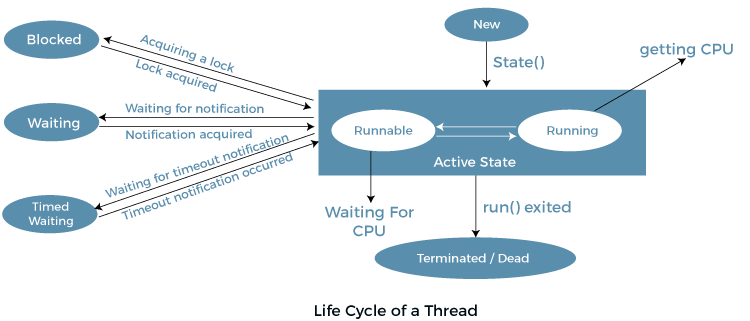
\includegraphics[width=1\textwidth]{src/img/life-cycle-of-a-thread.png}
  % \fromAuthor[width=\textwidth]{https://seeandselect.com/popedaze/life-cycle-of-a-thread}{life-cycle-of-a-thread.png}
  \fromAuthor[width=\textwidth]{https://static.javatpoint.com/core/images/life-cycle-of-a-thread.png}{life-cycle-of-a-thread.png}
\end{frame}

\begin{frame}[fragile]\frametitle{Nondeterministic thread execution}
~\\[-8mm]
\begin{columns}
\begin{column}{0.49\textwidth}
\begin{itemize}
  \item \texttt{``New thread''} printed always at the end
  \item Other prints not always in the same order -- nondeterministic execution
  \item Common in concurrent applications -- what makes it so hard
  \item Note: \texttt{join} also forces all memory writes from the threads before proceeding
\end{itemize}

\end{column}
\begin{column}{0.49\textwidth}
\begin{lstlisting}[emph={sleep,log,thread,join}]
object ThreadsNondeterminism extends App {
 val t = thread { log("New thread running.") }
     log("...")
     log("...")
     t.join()
     log("New thread joined.")
}
\end{lstlisting}
\end{column}
\end{columns}
\end{frame}


\section{Control of the execution order}

\begin{frame}[fragile]\frametitle{Atomic Execution}
\begin{itemize}
  \item \texttt{join} provides guarantees that other threads terminated
  \item Not enough -- we may want to inform other treads without terminating
\end{itemize}

\textbf{Example 1: shared counter for unique IDs}
\begin{lstlisting}[emph={sleep,log,thread,join}]
object ThreadsUnprotectedUid extends App {
  var uidCount = 0L
  def getUniqueId() = {
    val freshUid = uidCount + 1
    uidCount = freshUid
    freshUid
}
\end{lstlisting}

\structure{What can go wrong?}
\end{frame}


\begin{frame}[fragile]\frametitle{Atomic Execution}
~\\[-8mm]
\begin{columns}
\begin{column}{0.49\textwidth}
\begin{lstlisting}[emph={printUniqueIds,sleep,log,thread,join}]
...
def printUniqueIds(n: Int): Unit = {
  val uids = for (i<- 0 until n) yield getUniqueId()
  log(s"Generated uids: \§uids")
}
val t = thread { printUniqueIds(5) }
printUniqueIds(5)
t.join()
...
\end{lstlisting}
\end{column}
\begin{column}{0.49\textwidth}
\begin{lstlisting}[emph={sleep,log,thread,join}]
object ThreadsNondeterminism extends App {
 val t = thread { log("New thread running.") }
     log("...")
     log("...")
     t.join()
     log("New thread joined.")
}
\end{lstlisting}
\end{column}
\end{columns}
\only<1>{\structure{What do you expect?}}%
\only<2>{\begin{block}{Race Condition}
  when the \structure{output of a concurrent program} depends on \alert{how the statements are scheduled}.
\end{block}}
\end{frame}

\begin{frame}\frametitle{Updating counter in parallel}
  \centering
  \code{val freshUid = uidCount +  1 ;  uidCount = freshUid  ;  freshUid}

  \medskip
  
  \fromBookW{40}{26mm}{151mm}
\end{frame}

\begin{frame}[fragile]\frametitle{``Synchronized'' to the rescue}
~\\[-8mm]
\begin{columns}
\begin{column}{0.49\textwidth}
\begin{lstlisting}[emph={printUniqueIds,sleep,log,thread,join}]
def getUniqueId() =
   this.synchronized {
      val freshUid = uidCount + 1
      uidCount = freshUid
      freshUid
}
\end{lstlisting}
\end{column}
\begin{column}{0.49\textwidth}
\texttt{synchronized} is:
\begin{itemize}
  \item a fundamental Scala/Java construct for atomic executions
  \item can be called in \structure{any object} (or instance of a class)
  \item ensures atomic execution wrt the object
  \item we say \code{obj.synchronized}
    \begin{itemize}
      \item \alert{acquires} the \structure{lock/monitor} of \structure{obj} at the start
      \item \alert{releases} the \structure{lock/monitor} of \structure{obj} at the end
    \end{itemize}
\end{itemize}
\end{column}
\end{columns}
\end{frame}


\begin{frame}\frametitle{Updating counter in parallel atomically}
  \centering  
  \fromBookW{41}{26mm}{135mm}
\end{frame}

\begin{frame}%\frametitle{Life-cycle of a thread}
  \centering
  \fromAuthor[width=\textwidth]{https://static.javatpoint.com/core/images/life-cycle-of-a-thread.png}{life-cycle-of-a-thread.png}
\end{frame}


\begin{frame}\frametitle{Reordering}
\centering
\begin{itemize}
  \item using the \texttt{synchronized} statement has some (not too large) overhead
  \item not using \texttt{synchronized} can easily lead to errors, even if all seems correct
\end{itemize}

{\large \structure{Find the bug in the next slide...}}
\end{frame}


\begin{frame}[fragile]\frametitle{Find the bug}\label{slide:ThreadSharedStateAccessReordering}
\begin{lstlisting}[emph={assert,sleep,log,thread,join}]
object ThreadSharedStateAccessReordering extends App {
  for (i <- 0 until 100000) {
    var a = false
    var b = false
    var x = -1
    var y = -1
    val t1 = thread {
      a = true
      y = if (b) 0 else 1
    }
    val t2 = thread {
      b = true
      x = if (a) 0 else 1
    }
    t1.join()
    t2.join()
    assert(!(x==1 && y==1), s"x=\§x, y=\§y")
  }
}
\end{lstlisting}
\end{frame}


\begin{frame}\frametitle{Reordering within threads}
\begin{itemize}
  \item The previous code can raise an error: both \texttt{x} and \texttt{y} can become 1!

  \item JVM can reorder statements in a thread when they seem to be independent.

  \item Because some processors do not always execute instructions in the expected order, to increase performance.
  \item (Known as ``weak memory model'')
  \item A \texttt{synchronized} block would solve this:
    \begin{itemize}
      \item also enclosing each assignment in a \texttt{synchronized} block
      \item \texttt{synchronized} sets up a \emph{memory barrier} 
    \end{itemize}
\end{itemize}
\end{frame}




\begin{frame}[fragile]\frametitle{Locks and synchronization}
\begin{itemize}
  \item every object has a \emph{lock}
  \item a running \alert{thread} can \structure{aquire} multiple locks from different objects
\end{itemize}

\textbf{Example 2: Logging Bank Transfers}
\begin{lstlisting}[emph={assert,sleep,log,thread,join,synchronized}]
object SynchronizedNesting extends App {
   import scala.collection._
   
   private val transfers = mutable.ArrayBuffer[String]()
   def logTransfer(name: String, n: Int) = transfers.synchronized {
     transfers += s"transfer to account '\§name' = \§n"
   }
   class Account(val name: String, var money: Int)
   def add(account: Account, n: Int) = account.synchronized {
       account.money += n
       if (n > 10) logTransfer(account.name, n)
   }
   ...
}
\end{lstlisting}
\end{frame}


\begin{frame}[fragile]\frametitle{Locks and synchronization}
\begin{lstlisting}[emph={assert,sleep,log,thread,join,synchronized}]
   private val transfers = mutable.ArrayBuffer[String]()
   def logTransfer(name: String, n: Int) = transfers.synchronized {
     transfers += s"transfer to account '\§name' = \§n"
   }
   class Account(val name: String, var money: Int)
   def add(account: Account, n: Int) = account.synchronized {
       account.money += n
       if (n > 10) logTransfer(account.name, n)
   }

   val jane = new Account("Jane", 100)
   val john = new Account("John", 200)
   val t1 = thread { add(jane, 5) }
   val t2 = thread { add(john, 50) }
   val t3 = thread { add(jane, 70) } // will not corrupt Jane's account
   t1.join(); t2.join(); t3.join()
   log(s"--- transfers ---\n\§transfers")
\end{lstlisting}
\end{frame}


\section{Deadlocks}

\begin{frame}[fragile]\frametitle{Deadlocks -- the dark side of locks}

\begin{alertblock}{Deadlock}
  when two or more executions wait for each other before proceeding
\end{alertblock}

\begin{itemize}
  \item Studied in the first module with prof. Nelma Moreira
  \item \structure{Dining philosophers} is a typical example
  \item Often caused by locks that are not released at the right time
\end{itemize}

\begin{lstlisting}[emph={assert,sleep,log,thread,join,synchronized}]
object SynchronizedDeadlock extends App {
  import SynchronizedNesting.Account
  def send(a: Account, b: Account, n: Int) = a.synchronized {
    b.synchronized {
      a.money -= n
      b.money += n
    }
  }
  ... // can this go wrong?
}
\end{lstlisting}
\end{frame}


\begin{frame}[fragile]\frametitle{Deadlocks -- the dark side of locks}
\begin{lstlisting}[emph={assert,sleep,log,thread,join,synchronized}]
  def send(a: Account, b: Account, n: Int) = a.synchronized {
    b.synchronized {
      a.money -= n
      b.money += n
    }
  }

  val a = new Account("Jack", 1000)
  val b = new Account("Jill", 2000)
  val t1 = thread { for (i<- 0 until 100) send(a, b, 1) }
  val t2 = thread { for (i<- 0 until 100) send(b, a, 1) }
  t1.join(); t2.join()
  log(s"a = ${a.money}, b = ${b.money}")
\end{lstlisting}

{\Large \pause It works but... \pause \alert{it can deadlock}}
\end{frame}


\begin{frame}[fragile]\frametitle{Possible fix: fix order}

\begin{itemize}
  \item always acquire locks in the same order
  \item need a total order on locks
  \item we can use the getUniqueId (Example 1)
\end{itemize}
    
\begin{lstlisting}[emph={getUniqueId,sleep,log,thread,join,synchronized}]
import SynchronizedProtectedUid.getUniqueId
class Account(val name: String, var money: Int) {
  val uid = getUniqueId()
}
\end{lstlisting}
\pause
\begin{lstlisting}[emph={assert,sleep,log,thread,join,synchronized}]
def send(a1: Account, a2: Account, n: Int) {
  def adjust() {
    a1.money -= n
    a2.money += n
  }
  if (a1.uid < a2.uid)  a1.synchronized{ a2.synchronized{ adjust() }}
  else                  a2.synchronized{ a1.synchronized{ adjust() }}
}
\end{lstlisting}
\end{frame}

\section{Guarded blocks}

\begin{frame}\frametitle{Guarded blocks}
\begin{alertblock}{Guarded block (for us)}
  a \structure{block of code} that \alert{waits for a condition} before running in a thread
\end{alertblock}

\begin{block}{Example 3: Thread pool with a queue of tasks}
  \begin{itemize}
    \item Creating \structure{new threads} in Java is \alert{expensive} and \alert{avoidable}
    \item Usually we re-use threads, by maintaining a set of waiting threads
    \item This set is call a thread pool
      \begin{itemize}
        \item Scala already provides thread pools
        \item We first create our own
      \end{itemize}
  \end{itemize}
\end{block}
\end{frame}


\begin{frame}[fragile]\frametitle{}
~\\[-8mm]
\begin{columns}
\begin{column}{0.65\textwidth}
\begin{lstlisting}[emph={printUniqueIds,sleep,log,thread,join}]
 import scala.collection._
 object SynchronizedBadPool extends App {
  // our set of tasks
  private val tasks = mutable.Queue[()=>Unit]()
 
  // our single working thread
  val worker = new Thread {
    def poll(): Option[()=>Unit] = 
      asks.synchronized {
       if (tasks.nonEmpty) Some(tasks.dequeue())
       else                None
      }
    // keep on trying to run forever!
    override def run() = while (true)
      poll() match {
        case Some(task) => task()
        case None =>
    }
  }
\end{lstlisting}
\end{column}
\begin{column}{0.40\textwidth}
\begin{lstlisting}[emph={sleep,log,thread,join}]
  // starting the worker as a daemon
  worker.setName("Worker")
  worker.setDaemon(true)
  worker.start()

  def asynchr(body: =>Unit) =
    tasks.synchronized {
      tasks.enqueue(()=>body)
    }

  asynchr{ log("Hello")  }
  asynchr{ log(" world!")}
  Thread.sleep(5000)
}



$~$
\end{lstlisting}
\end{column}
\end{columns}
\end{frame}


\begin{frame}\frametitle{Note on daemon threads}
% \splittwo{
  \begin{alertblock}{Normal}
    \begin{itemize}
      \item not the default
      \item have lower priority
      \item terminated automatically when JVM terminates
      \item in other words, do not prevent the JVM from terminating
      \item (the JVM terminates when `normal' tasks terminate)
    \end{itemize}    
  \end{alertblock}
\end{frame}


\begin{frame}\frametitle{Bad busy-waiting}
    
  \begin{block}{Busy-waiting is bad}
    \begin{itemize}
      \item needlessly uses processor power (and drains the battery)
      \item after executing the previous code the \texttt{worker} will keep on running (unless you set in SBT \code{set fork := true},)
      \item in general, we want the \texttt{worker} to enter a waiting state
    \end{itemize}
    
  \end{block}
\end{frame}

\begin{frame}\frametitle{Avoiding busy-waiting}
\centering

{\Large \alert{synchronized} + \structure{wait} + \structure{notify}}

\begin{itemize}
  \item these are methods that every Java/Scala object has
  \item \structure{wait}:
    \begin{itemize}
      \item needs the lock
      \item puts the thread in a \alert{waiting} state
      \item releases the lock until activation
    \end{itemize}
  \item \structure{notify}:
    \begin{itemize}
      \item needs the lock
      \item \alert{activates} all waiting threads
    \end{itemize}
  \item Note that the JVM can decide to call \texttt{wait} on its own -- \alert{spurious wakeups} -- needing to re-enter the \emph{wait}
\end{itemize}
\end{frame}

\begin{frame}[fragile]\frametitle{Wait-notify example}
\begin{lstlisting}[emph={sleep,log,thread,join,wait,notify}]
object SynchronizedGuardedBlocks extends App {
  val lock = new AnyRef
  var message: Option[String] = None
  val greeter = thread {
    lock.synchronized {
      while (message == None) lock.wait() // non-busy waiting for a message
      log(message.get)                    // it will eventually log!
    }
  }
  lock.synchronized {
    message = Some("Hello!")
    lock.notify()                    // awakes the (possibly) locked thread
  }
  greeter.join()
}
\end{lstlisting}
\end{frame}


\begin{frame}[fragile]\frametitle{Example 3 -- without busy-waiting}
~\\[-8mm]
\begin{columns}
\begin{column}{0.65\textwidth}
\begin{lstlisting}[emph={printUniqueIds,sleep,log,thread,join,synchronized,wait,notify}]
import scala.collection._
object SynchronizedPool extends App {
  private val tasks = mutable.Queue[()=>Unit]()

  object Worker extends Thread {
    setDaemon(true)
    def poll() = tasks.synchronized {
      while (tasks.isEmpty) tasks.wait()
                         // now using wait
      tasks.dequeue()
    }
    override def run() = while (true) {
      val task = poll()
      task()
    }
  }
\end{lstlisting}
\end{column}
\begin{column}{0.40\textwidth}
\begin{lstlisting}[emph={sleep,log,thread,join,synchronized,wait,notify}]
  Worker.start()

  def asynchr(body: =>Unit) =
    tasks.synchronized {
       tasks.enqueue(()=>body)
       // now notifying
       tasks.notify()
    }

  asynchr{ log("Hello")  }
  asynchr{ log(" world!")}
  Thread.sleep(500)
}


$~$
\end{lstlisting}
\end{column}
\end{columns}


\end{frame}



\begin{frame}\frametitle{Interrupting threads -- \texttt{Thread.interrupt()}}
\begin{itemize}
  \item Our \texttt{Worker} can run forever (\texttt{while-true})
  \item Terminates when the JVM terminates (daemon)
  \item \texttt{Worker} can be terminated earlier while waiting
    \begin{itemize}
      \item \alert{\texttt{Worker.interrupt()}}
      \item triggers an \alert{\texttt{InterruptedException}} that can be handled
      \item if it was not waiting, then no exception is raised
      \item instead a flag \alert{\texttt{Worker.isInterrupted}} becomes true
    \end{itemize}
\end{itemize}
\end{frame}

\begin{frame}[fragile]\frametitle{Interrupting threads -- alternative with graceful shutdown}
    
\begin{lstlisting}[emph={sleep,log,thread,join,synchronized,wait,notify}]
object Worker extends Thread {
  var terminated = false
  // "manually" terminate when asked
  def poll(): Option[() => Unit] = tasks.synchronized {
    while (tasks.isEmpty && !terminated) tasks.wait()
    if (!terminated) Some(tasks.dequeue()) else None
  }

  import scala.annotation.tailrec
  @tailrec override def run() = poll() match {
    case Some(task) => task(); run()
    case None =>
  }
  // "manually" ask to terminate
  def shutdown() = tasks.synchronized {
    terminated = true
    tasks.notify()
  }
}
\end{lstlisting}

\end{frame}


\begin{frame}\frametitle{Volatile variables -- Alternative to \texttt{lock.synchronized}}
\begin{itemize}
  \item using the \texttt{\alert{@volatile}} annotation
  \\~
  \item can be atomically read and modified
  \item mostly used as status flag
  \item are never reordered in a thread
  \item writes are immediately visible to other threads
  \item very cheap to read
  \item not enough in many situations (e.g., \texttt{getUniqueID})
  \item enough for previous example -- Slide~\ref{slide:ThreadSharedStateAccessReordering}
\end{itemize}
\end{frame}

\begin{frame}[fragile]\frametitle{Example 4 -- Batman}
\begin{lstlisting}[emph={sleep,log,thread,join,synchronized,wait,notify,volatile}]
class Page(val txt: String, var position: Int)

object Volatile extends App {
  val pages = for (i<- 1 to 5) yield
    new Page("Na" * (100 - 20 * i) + " Batman!", -1)
  @volatile var found = false
  for (p <- pages) yield thread {
    var i = 0
    while (i < p.txt.length && !found)
      if (p.txt(i) == '!') {
        p.position = i
        found = true
      } else i += 1
  }
  while (!found) {}
  log(s"results: \§{pages.map(_.position)}")
}
\end{lstlisting}
\end{frame}


\section{The Java Memory Model overview}

\begin{frame}\frametitle{Happens-before relation}
\centering

\structure{action $\alpha$} \alert{happens-before} \structure{action $\beta$}\\
means  \structure{action $\beta$} sees the memory writes of \structure{action $\alpha$}

\begin{itemize}
\item \textbf{Program order:} $\alpha$ in a thread \alert{HB} every subsequent $\beta$ in that program and thread
\item \textbf{Monitor locking:} unlocking \alert{HB} every subsequent locking (of the same lock)
\item \textbf{Volatile fields:} writing to a volatile field \alert{HB} every of its subsequent read
\item \textbf{Thread start:} calling \texttt{thrd.start()} \alert{HB} any actions of \texttt{thrd}
\item \textbf{Thread termination:} $\alpha$ in a thread \alert{HB} a \texttt{join()} on that thread.
\item \textbf{Transitivity:} if $\alpha$ \alert{HB} $\beta$ and $\beta$ \alert{HB} $\gamma$, then a$\alpha$ \alert{HB} $\gamma$
\end{itemize}

\pause
\structure{Data race:} when a write to memory does not \alert{happen-before} its intended read.
\end{frame}

\begin{frame}[fragile]\frametitle{Immutable objects and final fields}
~\\[-8mm]
\begin{columns}
\begin{column}{0.42\textwidth}
\begin{lstlisting}[emph={printUniqueIds,sleep,log,thread,join,synchronized,wait,notify}]
class Foo(
  final val a: Int, val b: Int, c: Int)

class Foo { // Java code below
  final private int a\§;
  final private int b\§;
  final private int c\§;
  final public int a() {
    return a\§; }
  public int b() { return b\§; }
  public Foo(int a,
             int b,
             int c) {
    a\§ = a; b\§ = b; c\§ = c;
  }
}
\end{lstlisting}
\end{column}
\begin{column}{0.56\textwidth}
\begin{itemize}
  \item \structure{Final} fields: cannot be \alert{overridden}
  \item \structure{val}: cannot be \alert{updated}
  \item \structure{val}s are \structure{final}
  \item Some collections are immutable (e.g. \code{List}), but contain non-final fields
    \begin{itemize}
      \item need synchronisation when shared
    \end{itemize}
  \item Objects with only non-final fields
    \begin{itemize}
      \item do not need synchronisation when shared
    \end{itemize}
\end{itemize}
\end{column}
\end{columns}
\end{frame}

\begin{frame}[t]\frametitle{Summary of operators}
\begin{itemize}
  \item synchronize
  \item wait
  \item notify
  \item ...
\end{itemize}

\end{frame}

% \begin{frame}[fragile]\frametitle{Package objects}
% ~\\[-8mm]
% \begin{columns}
% \begin{column}{0.56\textwidth}
% \begin{lstlisting}
% package cp
% package object practical {
%   def log(msg: String): Unit =
%     println(s"${Thread.currentThread.getName}: $msg")
% }
% \end{lstlisting}
% \end{column}
% \begin{column}{0.42\textwidth}
% The \texttt{log} function is used throughout these lessons
% \end{column}
% \end{columns}
% \end{frame}


\end{document}
